\documentclass[mathNotesPreamble]{subfiles}
\begin{document}
%\relscale{1.4} %TODO
\section{15.5: Directional Derivatives and the Gradient}
  Directional derivatives allow us to evaluate the rate of change of a function $f(x,y)$ along any direction (not just parallel with the $x$-axis and $y$-axis).
  \vspace*{\stretch{1}}

  \begin{center}
    \hspace*{\stretch{1}}
    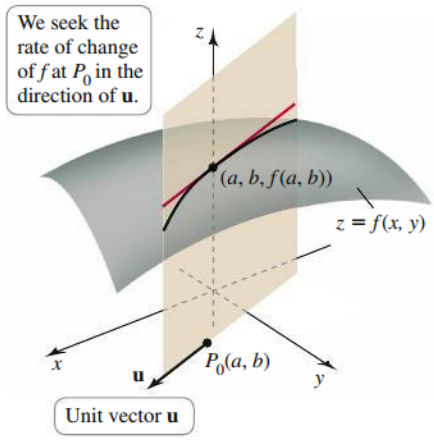
\includegraphics[width=0.375\linewidth]{images/briggs_15_05/fig15_45}
    \hspace*{\stretch{1}}
    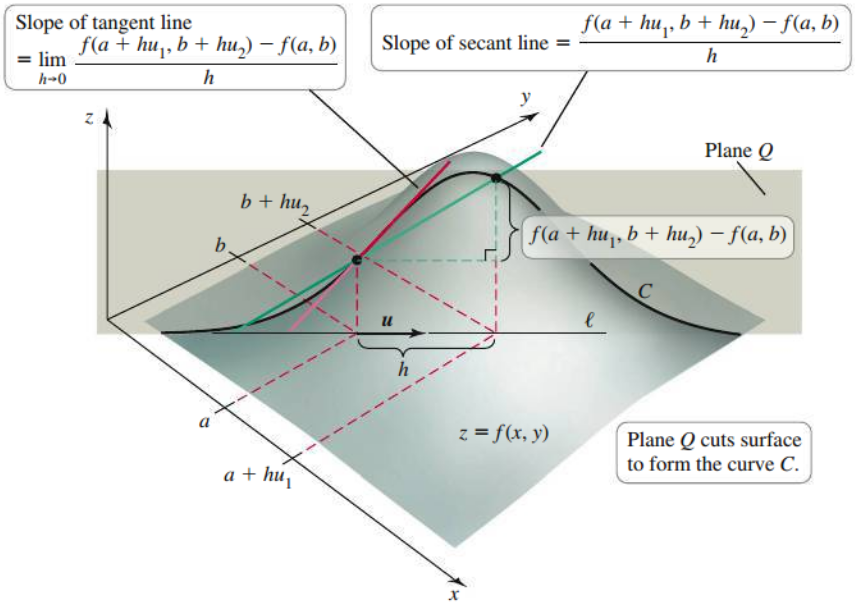
\includegraphics[width=0.55\linewidth]{images/briggs_15_05/fig15_47}
    \hspace*{\stretch{1}}
  \end{center}
  \vspace*{\stretch{1}}

  \begin{defn*}[Directional Derivative]
    Let $f$ be differentiable at $(a,b)$ and let $\vecu=\bracket{u_1,u_2}$ be a unit vector in the $xy$-plane. The \textbf{directional derivative of $f$ at $(a,b)$ in the direction of $u$} is 
      \[D_\vecu f(a,b)=\lim_{h\to 0} \frac{f(a+hu_1,b+hu_2)-f(a,b)}{h},\]
    provided the limit exists.
  \end{defn*}
  \pagebreak

  \noindent
  To motivate the formula for the directional derivative, let $\ell$ be a line going through $(a,b)$ in the direction of the unit vector $\vecu$. Now, let
  \vspace*{\stretch{1}}
    \[x=a+su_1,\quad\textnormal{ and }\quad y=b+su_2,\]

  \vspace*{\stretch{1}}
  where $-\infty<s<\infty$ and define
  \vspace*{\stretch{1}}
    \[g(s)=f(\underbrace{a+su_1}_x,\,\underbrace{b+su_2}_y),\]

  \vspace*{\stretch{1}}
  which evaluates $f$ along $\ell$. Thus, $g'(s)$ gives us the derivative along this line, and $g'(0)$ gives us the directional derivative of $f$ at $(a,b)$:
  \vspace*{\stretch{1}}
  \begin{align*}
    D_\vecu f(a,b)=g'(0)&=\left.\parens{\frac{\partial f}{\partial x}\smash{\underbrace{\frac{dx}{ds}}_{u_1}}+\frac{\partial f}{\partial y}\smash{\underbrace{\frac{dy}{ds}}_{u_2}}}\right|_{s=0}\\[0.75\baselineskip]
      &=f_x(a,b) u_1+f_y(a,b)u_2\\
      &=\bracket{f_x(a,b),\,f_y(a,b)}\cdot\bracket{u_1,u_2}.
  \end{align*}
  \vspace*{\stretch{1}}

  \noindent
  \fbox{\parbox{0.9875\linewidth}{
    \textbf{Theorem 15.10: Directional Derivative}\\
    Let $f$ be differentiable at $(a,b)$ and let $\vecu=\bracket{u_1,u_2}$ be a unit vector in the $xy$-plane. The \textbf{directional derivative of $f$ at $(a,b)$ in the direction of $\vecu$} is
      \[D_\vecu f(a,b)=\bracket{f_x(a,b), f_y(a,b)}\cdot\bracket{u_1, u_2}.\]
  }}
  \begin{center}
    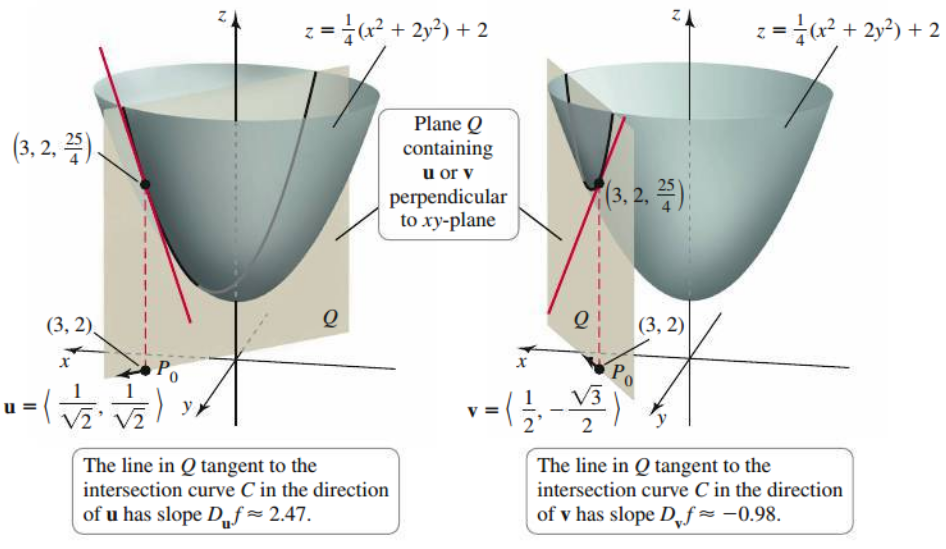
\includegraphics[width=0.55\linewidth]{images/briggs_15_05/fig15_48}
  \end{center}
  \pagebreak

  \begin{ex*}
    Compute the directional derivatives of the following functions at the given point along the given direction.
  \end{ex*}
  \begin{tasks}[after-item-skip=\stretch{1}, label=](1)
    \task $f(x,y)=\sqrt{4-x^2-2y}$; $P(2,-2)$; and $\vecu=\bracket{\frac{1}{\sqrt{10}},\,\frac{3}{\sqrt{10}}}$,
    \task $g(x,y)=\tan\inv(xy)$; $P(\pi,1/3)$; along $\vecu=\bracket{1,1}$,
    \task $h(x,y)=2x^2-xy+3y^2$; $P(1,-3)$; along $\vecu=\bracket{1,-1}$ and $\vecv=\bracket{\frac{3}{5},\,\frac{4}{5}}$.
  \end{tasks}
  \vspace*{\stretch{1.5}}
  \pagebreak

  \noindent
  \textbf{The Gradient Vector:}\\
  The vector of derivatives used in the directional derivative is called the \textit{gradient} of $f$.
  \begin{defn*}[Gradient (Two Dimensions)]
    Let $f$ be differentiable at the point $(x,y)$. The \textbf{gradient} of $f$ at $(x,y)$ is the vector-valued function
      \[\grad f(x,y)=\bracket{f_x(x,y),\,f_y(x,y)}=f_x(x,y)\bfi+f_y(x,y)\bfj.\]
  \end{defn*}

  \begin{ex*}
    For $\ds f(x,y)=3-\frac{x^2}{10}+\frac{xy^2}{10}$, compute $\grad f(3,-1)$, then compute $D_\vecu f(3,-1)$, where $\ds\vecu=\bracket{\frac{1}{\sqrt{2}},-\frac{1}{\sqrt{2}}}$.
  \end{ex*}
  \vspace*{\stretch{1}}

  \noindent
  \fbox{\parbox{0.9875\linewidth}{
    \textbf{Theorem 15.11: Directions of Change}\\
    Let $f$ be differentiable at $(a,b)$ with $\grad f(a,b)\neq \bfO$.
    \begin{enumerate}
      \item 
        $f$ has its maximum rate of increase at $(a,b)$ in the direction of the gradient $\grad f(a,b)$. The rate of change in this direction is $\abs{\grad f(a,b)}$.
      \item 
        $f$ has its maximum rate of decrease at $(a,b)$ in the direction of $-\grad f(a,b)$. The rate of change in this direction is $-\abs{\grad f(a,b)}$.
      \item 
        The directional derivative is zero in any direction orthogonal to $\grad f(a,b)$.
    \end{enumerate}
  }}
  \pagebreak

  \begin{ex*}
    For $f=4+x^2+3y^2$: 
  \end{ex*}
  \begin{tasks}[after-item-skip=\stretch{1}, label=](1)
    \task What direction is the greatest ascent at $P(2,-\frac{1}{2}, \frac{35}{4})$? What is the rate of change in this direction?
    \task What direction is the greatest descent at $P(\frac{5}{2},-2, \frac{89}{4})$? What is the rate of  change in this direction?
    \task What direction results in no change in function values at $P(3,1, 16)$?
  \end{tasks}
  \vspace*{\stretch{1}}
  \pagebreak

  \noindent
  \fbox{\parbox{0.9875\linewidth}{
    \textbf{Theorem 15.12: The Gradient and Level Curves}\\
    Given a function $f$ differentiable at $(a,b)$, the line tangent to the level curve of $f$ at $(a,b)$ is orthogonal to the gradient $\grad f(a,b)$, provided $\grad f(a,b)\neq \bfO$.
  }}

  \noindent
  \begin{minipage}{0.6\linewidth}

    \textit{Note:} From Theorem 15.12, we get an equation for the line tangent to the curve $z=f(x,y)$ at $(a,b)$:
      \[\grad f(a,b)\cdot\bracket{x-a,\,y-b}=0.\]
  \end{minipage}%
  \hspace*{\stretch{1}}
  \begin{minipage}{0.3\linewidth}
    \begin{flushright}
      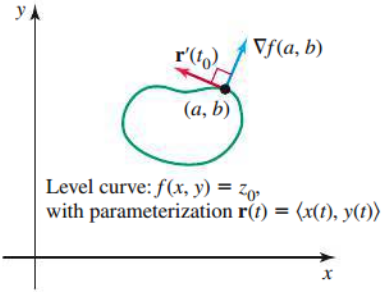
\includegraphics[width=\linewidth]{images/briggs_15_05/fig15_53}
    \end{flushright}
  \end{minipage}

  \begin{ex*}
    Consider the upper sheet $z=f(x,y)=\sqrt{1+2x^2+y^2}$ of a hyperboloid of two sheets.
  \end{ex*}
  \begin{tasks}[after-item-skip=\stretch{1}, label=](1)
    \task Verify that the gradient at $(1,1)$ is orthogonal to the corresponding level curve at that point.
    \task Find an equation of the line tangent to the level curve at $(1,1)$.
  \end{tasks}
  \vspace*{\stretch{0.5}}

  \pagebreak

  \begin{ex*}
    Consider $\ds z=f(x,y)=15-\frac{x^2}{25}-\frac{y^2}{9}$:
  \end{ex*}
  \begin{tasks}[after-item-skip=\stretch{1}, label=](1)
    \task Compute the slope of the tangent line at $P(5\sqrt{5},-6,6)$.
    \task Verify the gradient is orthogonal to the tangent line.
  \end{tasks}
  \vspace*{\stretch{0.5}}
  \pagebreak

  \begin{defn*}[Directional Derivative and Gradient in Three Dimensions]
    Let $f$ be directional at $(a,b,c)$ and let $\vecu=\bracket{u_1,\,u_2,\,u_3}$ be a unit vector. The \textbf{directional derivative of $f$ at $(a,b,c)$ in the direction of $\vecu$} is
      \[D_\vecu (a,b,c)=\lim_{h\to 0} \frac{f(a+hu_1,\,b+hu_2,\,c+hu_3)-f(a,b,c)}{h},\]
    provided this limit exists.\newline
    The \textbf{gradient} of $f$ at this point $(x,y,z)$ is the vector-valued function
      \begin{align*}
        \grad f(x,y,z)&=\bracket{f_x(x,y,z),\,f_y(x,y,z),\,f_z(x,y,z)}\\
          &=f_x(x,y,z)\bfi+f_y(x,y,z)\bfj+f_z(x,y,z)\bfk.
      \end{align*}
  \end{defn*}
  \vspace*{\stretch{1}}

  \noindent
  \fbox{\parbox{0.9875\linewidth}{
    \textbf{Theorem 15.13: Directional Derivative and Interpreting the Gradient}\\
    Let $f$ be differentiable at $(a,b,c)$ and let $\vecu=\bracket{u_1,\,u_2,\,u_3}$ be a unit vector. The directional derivative of $f$ at $(a,b,c)$ in the direction of $\vecu$ is
    \begin{align*}
      D_\vecu f(a,b,c)&=\grad f(a,b,c)\cdot \vecu\\
        &=\bracket{f_x(a,b,c),\, f_y(a,b,c),\,f_z(a,b,c)}\cdot\bracket{u_1,\,u_2,\,u_3}.
    \end{align*}
    Assuming $\grad f(a,b,c)\neq \bfO$, the gradient in three dimensions has the following properties.
    \begin{enumerate}
      \item 
        $f$ has its maximum rate of increase at $(a,b,c)$ in the direction of the gradient $\grad f(a,b,c)$ and the rate of change in this direction is $\abs{\grad f(a,b,c)}$.
      \item 
        $f$ has its maximum rate of decrease at $(a,b,c)$ in the direction of $-\grad f(a,b,c)$ and the rate of change in this direction is $-\abs{\grad f(a,b,c)}$.
      \item 
        The directional derivative is zero in any direction orthogonal to $\grad f(a,b,c)$.
    \end{enumerate}
  }}
  \pagebreak

  \begin{ex*}
    Consider $f(x,y,z)=x^2+2y^2+4z^2-1$ and the level surface $f(x,y,z)=3$. Find the gradient and the corresponding rate of change at the points $P(2,0,0)$, $Q(0,\sqrt{2},0)$, $R(0,0,1)$, and $S(1,1,1/2)$ on the level surface.
  \end{ex*}

  \pagebreak
  
\end{document}
